\begin{figure}
\centering
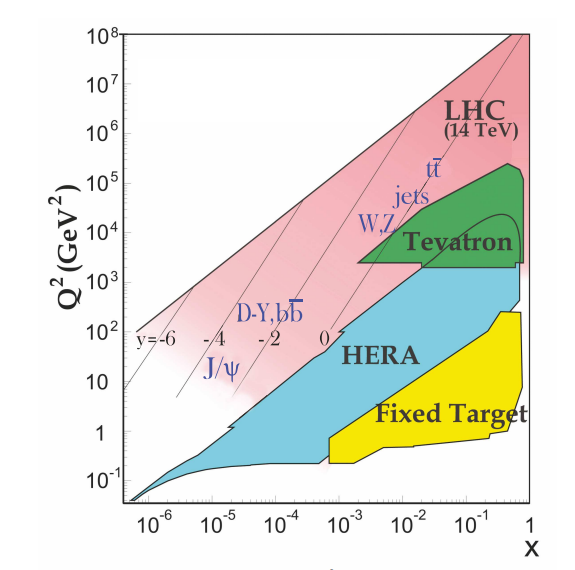
\includegraphics[width=0.6\linewidth]{plots/SM/structure_probes.PNG}
%   \caption{1a}
%   \label{fig:Eff:el:5TeV:GSFSel:pos
\caption{Phase space of Bjorken-x and $Q^2$ available at the LHC and other experiments. Proton-proton collisions at the LHC can probe very high $Q^2$. With an acceptance of $|y| < 2.4$, \W and \Z boson cross section measurements can probe approximately $10^-4 < x < 0.1$ \protect\cite{PhysRevD.98.030001}}
\label{fig:sm:summary:xVsQ2}
\end{figure}